\section{Data Recap}

\begin{figure}
    \centering
    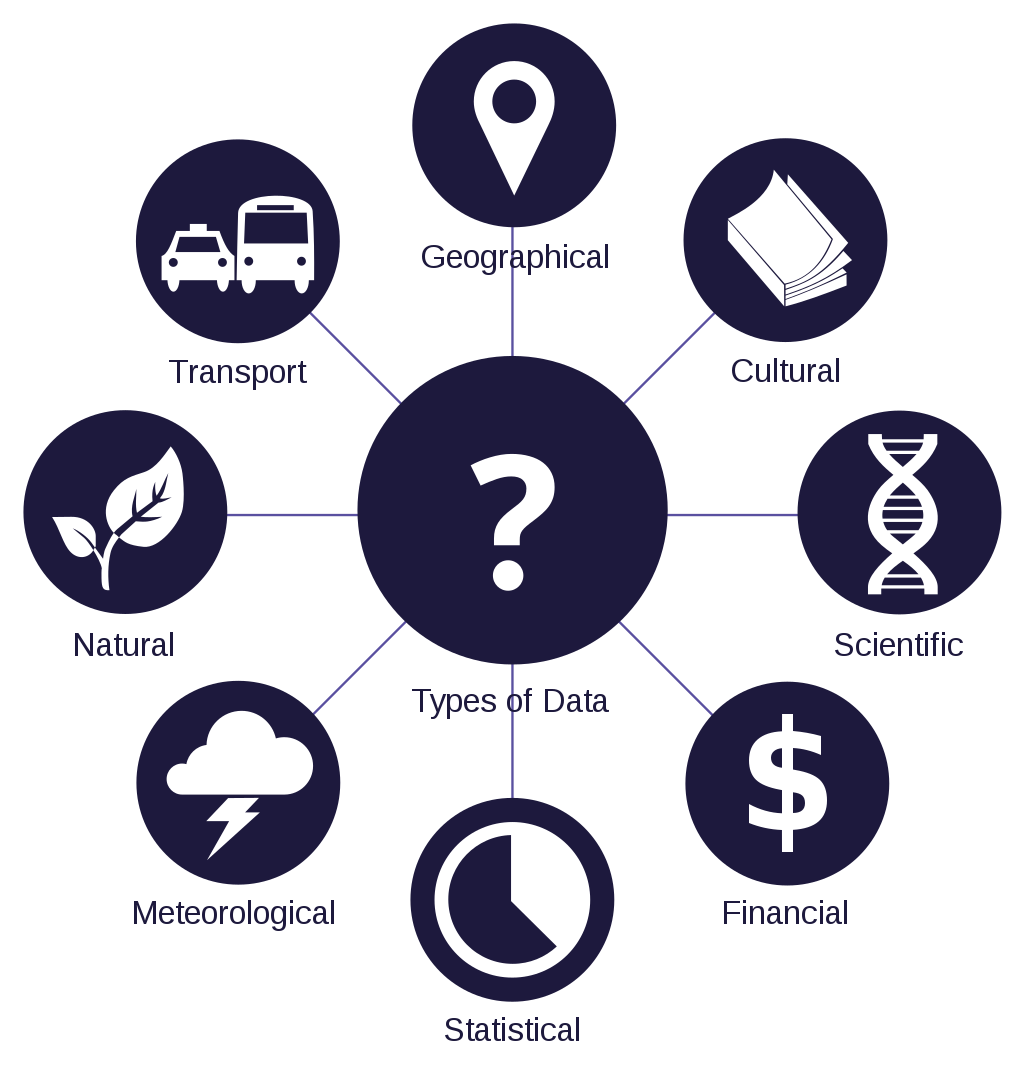
\includegraphics[width=0.5\linewidth]{figures/datatypespng.png}
    \caption{Different kinds of data.}
    \label{fig:datatypes}
\end{figure}

Data is units of information, and in a technical perspective, data is a set
of values of quantitative or qualitative variables about a data object. 
Data should be understood in the context of information. Information can be 
thought of as the resolution of uncertainty, though it's 
exact interpretation and meaning differs in different context. Using this
vague definition of information it becomes clear how diverse data can be.
Just see figure \ref{fig:datatypes} for examples. 
Everything that removes uncertainty contains information and can potentially 
be stored and processed as data.

\subsection{Difference between data and information.}
Data and Information is often talked about interchangably but are two different
things or rather two different levels of abstraction of the same thing. Data is 
a structured or unstructured collection of symbols. Information resolves 
uncertainty and does not take any particular form. Data can represent reduntant
symbols but can be said to approach information through optimal compression. 
One of the most common ways to structure data is to have a set of data objects
and their attributes.

\section{Attributes}
\begin{itemize}
    \item An attribute is a property or characteristic of an object
    \begin{itemize}
        \item Attribute are also known as variables, fields, characteristics, or features
    \end{itemize}
    \item A collection of attributes describe an object
    \begin{itemize}
        \item Objects are also known as records, points, cases, samples, entries, or instances
    \end{itemize}
\end{itemize}

\subsection{Values}
Attribute values are numbers or symbols assigned to an attribute.
The distinction between attributes and attribute values are:
\begin{itemize}
    \item Same attribute can be mapped to different attribute values
    \item Different attributes can be mapped to the same set of values
\end{itemize}

\subsection{Types}
\begin{center}
    \begin{table}[H]
        \begin{tabular}{l|l|l}
            \begin{tabular}[c]{@{}l@{}}
                Attribute \\Type
            \end{tabular}&
            Operations &
            Transformations \\ \hline \hline
        \begin{tabular}[c]{@{}l@{}}
            \\Nomial\\ \\
        \end{tabular}&
            \begin{tabular}[c]{@{}l@{}}
                Mode, Entropy, Contingency, \\
                Correlation, $\chi^2$-test
            \end{tabular}&
            \begin{tabular}[c]{@{}l@{}}
                Any permutation of values
            \end{tabular} \\ \hline
        \begin{tabular}[c]{@{}l@{}}
            \\Ordinal\\ \\
        \end{tabular}&
            \begin{tabular}[c]{@{}l@{}}
                Median, Rank correlation, \\
                Percentiles, Run tests, Sign tests
            \end{tabular}&
            \begin{tabular}[c]{@{}l@{}}
                Order-preserving change of values\\
                $new\_value = f(old\_value)$ \\
                where $f$ is a monotonic function.
            \end{tabular} \\ \hline
        \begin{tabular}[c]{@{}l@{}}
            \\Interval\\ \\
        \end{tabular}&
            \begin{tabular}[c]{@{}l@{}}
                Mean, Standard deviation, $t$-tests\\
                Pearson's correlation, $F$-tests
            \end{tabular}&
            \begin{tabular}[c]{@{}l@{}}
                $new\_value = a * old\_value + b$ \\
                where a and b are constants
            \end{tabular} \\ \hline
        \begin{tabular}[c]{@{}l@{}}
            \\Ratio\\ \\
        \end{tabular}&
            \begin{tabular}[c]{@{}l@{}}
                Geometric mean, Harmonic mean, \\
                Percent variation
            \end{tabular}&
            \begin{tabular}[c]{@{}l@{}}
                $new\_value = a * old\_value$
            \end{tabular}
        \end{tabular}
    \end{table}
\end{center}

\subsection{Discrete and Continuous Attributes}
Discrete attributes:
\begin{itemize}
    \item Finite or countably infinite set of values
    \item Often integer or binary variables
\end{itemize}

Continuous attributes:
\begin{itemize}
    \item Real numbers as attribute values
    \item Typically floating-point variables
\end{itemize}

\section{Datasets}
Some important characteristics of structured data are:
\begin{itemize}
    \item Dimensionality
    \begin{itemize}
        \item Curse of dimensionality
        \begin{itemize}
            \item As the number of features or dimensions grow, the amount of data needed to generalize accurately grows exponentially.
            \item When data moves from one dimensions to i.e. three dimensions, the given data fills less and less of the data space.
                  In order to maintain an accurate representation of the space, the data for analysis grows exponentially.
            \item When sorting or classifying data, low dimensional spaces tend to show the data as very similar,
                  but in higher dimensions, the data might be further away from each other.
        \end{itemize}
    \end{itemize}
    \item Sparsity
    \begin{itemize}
        \item Only presence counts
    \end{itemize}
    \item Resolution
    \begin{itemize}
        \item Patterns depend on the scale
    \end{itemize}
\end{itemize}

\subsection{Record Data}
Data that consists of a collection of records, each of which consists of a fixed set of attributes.

\subsubsection{Data Matrix}
If data objects have the same fixed set of numeric attributes, then the data objects can be thought of as points in a multi-dimensional space, where each dimension represents a distinct attribute.
Such data set can be represented by an $m$ by $n$ matrix, where there are $m$ rows, one for each object, and $n$ columns, one for each attribute.

\subsubsection{Document Data}
Each document becomes a \textit{term} vector.
Each term is a component (attribute) of the vector.
The value of each component is the number of times the corresponding term occurs in the document.

\subsubsection{Transaction Data}
A special type of record data, where each record (transaction) involves a set of items.
For example, consider a grocery store. The set of products purchased by a customer during one shopping trip constitute a transaction, while the individual products that were purchased are the items.

\subsection{Graph Data}
Data which can be represented as a collection of edges and vertices. 
I.e. chemical structures. Graph data can be directional or undirectional. 

\subsection{Sequential Data}
Data in which sequence matters. One cannot permutate the data in a meaningful
way. I.e. time series data or gene sequences.

\subsection{Spatio-temporal Data}
This is data that represents information about both space and time. 
I.e average temperatures in the world. 

\section{Data Quality}

Data Quality is important to measure, detect and improve. Data is elevated to 
information when optimal data compression is achieved. Problems that reduce the
quality of data threatens to damage or skew the information the data is supposed
to represent. There are many examples of data quality problems and some of them 
are adressed in this section.

\subsection{Noise}
Ultimately, Noise can be throught as $\epsilon$ in the following equation

\begin{equation}
    D = S + \epsilon
\end{equation}

Where $D$ is the colleted Data and $S$ is the true signal. Noise is therefore a 
modification of original / correct values.

\subsection{Outliers}
Outliers are data objects with characteristics that are considerably different 
than most of the other data objects in the data set. Though outliers are 
theorietically possible in many distributions (i.e Normal Distribution) outliers
indicate some experimental error or heavy tails. In the former case one either
discard the outliers completely or use robust statistics or in the latter case
be careful in using statistical tests that assume normal distributions.

\subsection{Missing Values}
Reasons for missing values may be that some information is not collected or 
applicable to all cases.

Handling missing values can be done by:

\begin{itemize}
    \item Eliminating data objects
    \item Estimating the missing values
    \item Ignoring the missing values during analysis
    \item Replacing the missing values with all possible values weighted by 
    their probabilities
\end{itemize}

\subsection{Duplicate Data}
Data set may include data objects that are duplicates, or almost duplicates of 
one another. This is a major issue when merging data from heterogenous sources.

\section{Distance/Similarity Functions}
According to \cite{enwiki:similarity}:

\medskip
In statistics and related fields, a similarity measure or similarity function is 
a real-valued function that quantifies the similarity between two objects. 
Although no single definition of a similarity measure exists, usually such 
measures are in some sense the inverse of distance metrics: they take on large 
values for similar objects and either zero or a negative value for very 
dissimilar objects. 

\begin{itemize}
    \item Similarity
    \begin{itemize}
        \item Numerical measure of how alike two data objects are
        \item Higher value means more alike
        \item Often falls in the range $[0,1]$
    \end{itemize}
    \item Dissimilarity
    \begin{itemize}
        \item Numerical measure of how different two data objects are
        \item Lower when objects are more alike
        \item Minimum dissimilarity is often 0
        \item Upper limit varies
    \end{itemize}
    \item Proximity refers to a similarity or dissimilarity
\end{itemize}

\subsection{Similarity/Dissimilarity for Simple Attributes}
Given that $p$ and $q$ are the attribute values for two data objects:
\begin{center}
    \begin{table}[H]
        \begin{tabular}{l|l|l}
            Attribute Type &
            Dissimilarity &
            Similarity \\ \hline \hline

            Nominal &
            $d = \left\{\begin{matrix} 0 & if & p=q\\  1 & if & p \neq q \end{matrix}\right.$ &
            $s = \left\{\begin{matrix} 1 & if & p=q\\  0 & if & p \neq q \end{matrix}\right.$ \\ \hline

            Ordinal &
            $d = \frac{|p-q|}{n-1}$&
            $s = 1 - \frac{|p-q|}{n-1}$ \\ \hline

            Interval/Ratio &
            $d = |p-q|$&
            $s = -d$, $s = \frac{1}{1+d}$, $s = 1- \frac{d- min(d)}{max(d)-min(d)}$
        \end{tabular}
    \end{table}
\end{center}

\subsection{Euclidean distance}

Euclidean distance is defined in the following theorem, where $n$ 
is the number of dimensions (attributes) and $p_k$ and $q_k$ are, respectively,
the $k_th$ attributes (components) or data objects $p$ and $q$.

\begin{theo}[Euclidean Distance]{theo:theo1}
\label{eq:euclidean-distance}
The distance between two points in Euclidean space 
is the length of a line segment between the two points. It can be calculated 
from the Cartesian coordinates of the points using the Pythagorean theorem. 
In $n$ dimensions:
    \[
        distance = \sqrt{\sum_{k=1}^{n}(p_k-q_k)^2}
    \]
\end{theo}

Standarization is necessary if scales differ.


\subsection{Minkowski Distance}

Minkowski Distance is a generalization of Euclidean Distance where
$r$ is a parameter, $n$ is the number of dimensions (attributes) and $p_k$ and $q_k$ are, 
respectively, the $k_th$ attributes (components) or data objects $p$ and $q$.

\begin{theo}[Minkowski Distance]{theo:theo2}
\label{eq:minkowski-distance}
    \[
        distance = \sqrt[r]{\sum_{k=1}^{n}|p_k-q_k|^r}
    \]
\end{theo}

\begin{itemize}
    \item $r = 1$: Manhattan distance
    \item $r = 2$: Manhattan distance
    \item $r \rightarrow \infty$: "Supremum" distance
    \begin{itemize}
        \item This is the maximum difference between any component of the vectors
    \end{itemize}
\end{itemize}

\subsection{Properties of Distance Functions}
Distances, such as the Euclidean distance, have some well known properties.
\begin{itemize}
    \item Positive definiteness
    \begin{itemize}
        \item $d(p, q) \geq 0$ for all $p$ and $q$
        \item $d(p, q) = 0$ only if $p = q$
    \end{itemize}
    \item Symmetry
    \begin{itemize}
        \item $d(p, q) = d(q, p) 0$ for all $p$ and $q$
    \end{itemize}
    \item Triangle Inequality
    \begin{itemize}
        \item $d(p, r) \leq d(p, q) + d(q, r)$ for all $p$. $q$ and $r$
    \end{itemize}
\end{itemize}

\begin{lem}[Metric]{lem:leml}
    A distance that satisfies the properties mentioned above is a metric.
\end{lem}

\subsection{Properties of Similarity Functions}
Well known properties of similarities.
\begin{itemize}
    \item Maximum Similarity
    \begin{itemize}
        \item $s(p, q) = 1$ (or maximum similarity) only if $p = q$
    \end{itemize}
    \item Symmetry
    \begin{itemize}
        \item $s(p, q) = s(q, p) 0$ for all $p$ and $q$
    \end{itemize}
\end{itemize}

\section{Similarity/Coefficient}
A common situation is that objects, $p$ and $q$, have only binary attributes.

Let's define:
\begin{itemize}
    \item $M_{01}$ - Number of attributes where $p$ is 0 and $q$ is 1
    \item $M_{10}$ - Number of attributes where $p$ is 1 and $q$ is 0
    \item $M_{00}$ - Number of attributes where $p$ is 0 and $q$ is 0
    \item $M_{11}$ - Number of attributes where $p$ is 1 and $q$ is 1
\end{itemize}


\subsection{Simple Matching Coefficient}

\begin{equation}
    SMC = \frac{\text{Number of matches}}{\text{Number of attributes}}
\end{equation}
\begin{equation}
    SMC = \frac{M_{00} + M_{11}}{M_{01} + M_{10} + M_{00} + M_{11}}
\end{equation}


\subsection{Jaccard Similarity/Coefficient}

The Jaccard Similarity/Coefficient is used for categorical attributes and sets.

\begin{equation}
    J = \frac{\text{Number of } M_{11}}{\text{Number of non-both-zero attributes}}
\end{equation}
\begin{equation}
    J = \frac{M_{11}}{M_{01} + M_{10} + M_{11}}
\end{equation}

\begin{equation}
    J(A, B) = \frac{|A \cap B|}{|A \cup B|} = \frac{|A \cap B|}{|A|+|B|-|A \cup B|}
\end{equation}

\subsection{Cosine Similarity}
If $\bm{A}$ and $\bm{B}$ are two documented vectors, then

\begin{equation}
    \text{similarity} = \cos(\theta) = \frac{\bm{A}\cdot\bm{B}}{\norm{\bm{A}} \norm{\bm{B}}} =
    \frac{\sum_{i=1}^n A_i B_i}{\sqrt{\sum_{i=1}^n A_i^2} \sqrt{\sum_{i=1}^n B_i^2}}
\end{equation}

\section{Dot Product}
Given two vectors $a$ and $b$:

\begin{equation}
    \overrightarrow{a} \cdot \overrightarrow{b} = \sum_{i=1}^n a_i b_i =
    a_1 b_1 + a_2 b_2 + \cdots + a_n b_n 
\end{equation}

\section{Data Preprocessing}
\subsection{Aggregation}
Aggregation is to combine two or more attributes (or objects) into a single attribute \\(or object).

\medskip
Purpose:
\begin{itemize}
    \item Data reduction
    \item Reduce the number of attributes or objects
    \item Change of scale
    \item More "stable" data
    \item Often reduce variability
\end{itemize}

\subsection{Data Sampling}
Data sampling is the main technique employed for data selection.
It is often used for both the preliminary investigation of the data and the final data analysis.
Statisticians sample because obtaining the entire set of data of interest is too expensive or time consuming.
Sampling is used in data mining because processing the entire set of data of interest is too expensive or time consuming.
A good stategy for choosing the sample size is to aim for a sample size that is 10$\%$ of the population, as long as the sample size is smaller than 1000.
It is also important to have a large enough sample size so that all attributes/groups are represented.

\medskip
Sampling is effective when:
\begin{itemize}
    \item The sample is representative
    \item The sample has approximately the same properties (of interest) as the original set of data
\end{itemize}

\medskip
Types of sampling:
\begin{itemize}
    \item Simple random sampling
    \begin{itemize}
        \item Equal probability of selecting any item.
    \end{itemize}
    \item Sampling without replacement
    \begin{itemize}
        \item As each item is selected, it is removed from the population.
    \end{itemize}
    \item Sampling with replacement
    \begin{itemize}
        \item Objects are not removed from the population as they are selected for the sample.
    \end{itemize}
    \item Stratified sampling
    \begin{itemize}
        \item Split the data into several partitions, then draw random samples from each partition.
    \end{itemize}
\end{itemize}

\subsubsection{Reservoir Sampling}

\textbf{The problem:}
\medskip
We want to perform a simple random sample (uniform random sample) on a 
continuous stream of data of unknown size. Reservoir sampling achieves this.

\begin{theo}[Reservoir Sampling]{theo:theo3}
    \label{eq:reservoir-sampling}
        Keep a reservoir of $r$ samples
        \begin{enumerate}
            \item Keep the first $r$ items in memory
            \item When the $i^{th}$ item arrives $(i>r)$
            \begin{enumerate}
                \item Keep the new item with probability $\frac{r}{i}$, \\
                or discard the new item with probability $1 - \frac{r}{i}$
                \item Discard one of the items in the reservoir at random \\
                if the new item was kept.
            \end{enumerate}
        \end{enumerate}

    This means that as $i$ increases, the probability of a new item being kept in the reservoir reduces.
\end{theo}

\section{Dimensionality Reduction}
\begin{itemize}
    \item Purpose
    \begin{itemize}
        \item Avoid curse of dimensionality
        \item Reduce amount of time and memory required by data mining
        \item Allow data to be more easily visualized
        \item May help eliminate irrelevant features or reduce noise
    \end{itemize}
    \item Techniques
    \begin{itemize}
        \item Pronciple Component analysis
        \item Singular Value Decomposition
    \end{itemize}
\end{itemize}
